\subsection{FPGA}


The FPGA (Field Programmable Gate Array) is a circuit that contains multiple logic blocks and routing channels.\\
The hardware configuration is customizable in order to meet the user’s demands in the digital domain; unlike ICs where the connections between the transistors cannot be changed, it is possible to make a custom architecture on an FPGA. \\
As said, the FPGA consists of multiple logic blocks often called logic cells. Each cells consists of an LUT (Look-up table) and a flip-flop. The LUT has four inputs and the flip-flop one clock input. The LUT contains a small Random Access Memory and performs logical operation. \\
Around the logic blocks, there are multiple I/O blocks which can also be programmed to an output or input for instance.  \\
An FPGA contains a configuration logic that is connected to the flash memory which contains information about the connection between the logic blocks and the architecture inside the block itself. The more logic blocks are used and programmed, the bigger the flash memory storage size has to be. An overview of the structure of the FPGA is shown in \autoref{fig:fpgastructure} and the structure of the logic block in \autoref{fig:logicblockstruct}. \\
\newline

\begin{figure}[htbp]
	\centering
	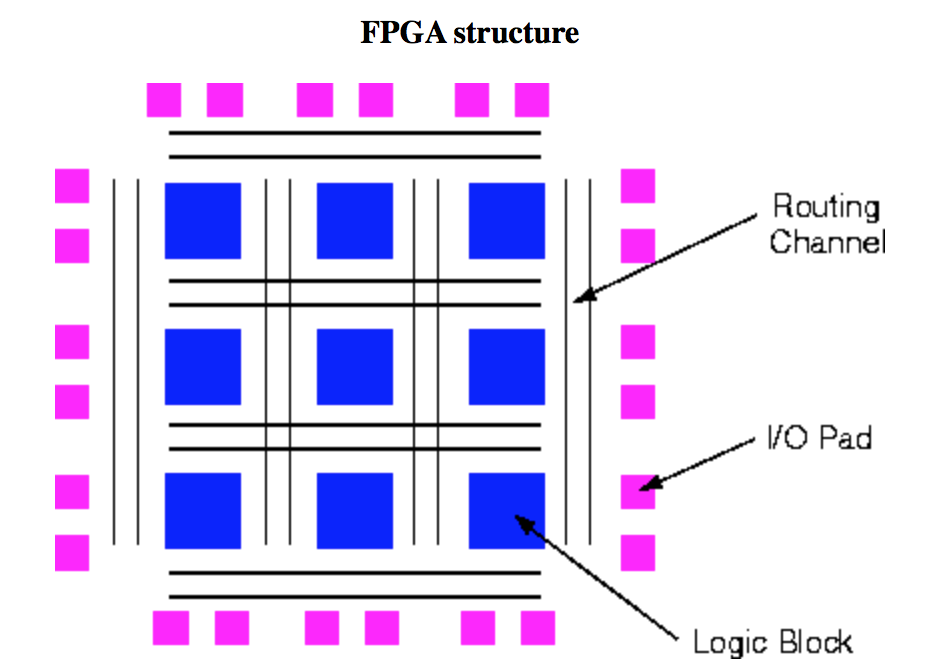
\includegraphics[width=0.7\textwidth]{fpgastructure}
	\caption{Scheme of FPGA components.}
	\label{fig:fpgastructure}
\end{figure}

\begin{figure}[htbp]
	\centering
	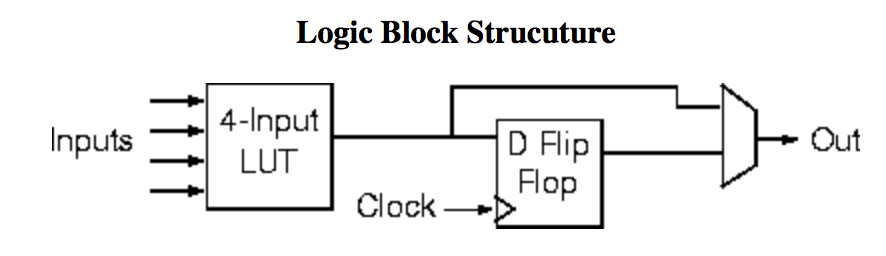
\includegraphics[width=0.7\textwidth]{logicblockstruct}
	\caption{Structure of a logic block.}
	\label{fig:logicblockstruct}
\end{figure}


The biggest advantage of the FPGA is to make multiple processes at the same time by isolating some logic blocks and I/Os for a specific task, which is not possible with ICs. A micro controller needs to run tasks in sequence, one after the other. If different tasks needs to be done in a restricted timing, this parameter can be crucial. 
By using parallelism and having fast I/Os, the FPGA can be very powerful. \\

The FPGA can be programmed using a hardware description language like VHDL or Verilog. \\

FPGA are certainly more efficient than ICs and normal micro controller but they are also more expensive especially if it’s about cloning a pre-existing micro controller without any personal added value. They are also power demanding. The FPGA has a configuration flash memory which means that there is no need for the user to intervene after a reboot, but at each boot the FPGA is programmed from scratch using the data from the flash memory which can drastically increase the boot time as well as the power consumption. It is more complicated to program an FPGA than using an IC or micro controller because it has to be designed by the user. \\








